\documentclass{article}
\newsavebox{\oldepsilon}
\savebox{\oldepsilon}{\ensuremath{\epsilon}}
\usepackage[minionint,mathlf,textlf]{MinionPro} % To gussy up a bit
\renewcommand*{\epsilon}{\usebox{\oldepsilon}}
\usepackage[margin=1in]{geometry}
\usepackage{graphicx} % For .eps inclusion
%\usepackage{indentfirst} % Controls indentation
\usepackage[compact]{titlesec} % For regulating spacing before section titles
\usepackage{adjustbox} % For vertically-aligned side-by-side minipages
\usepackage{array, amsmath,  mhchem}
\usepackage[hidelinks]{hyperref}
\usepackage{courier, subcaption}
\usepackage{multirow, enumerate}

\usepackage{float}
\restylefloat{table}

\pagenumbering{gobble} 
\setlength\parindent{0 cm}
\renewcommand{\arraystretch}{1.2}
\begin{document}
\large

MCB 135 Problem Set 2 \hfill Due Wednesday, February 18, 2015 at 2:30 PM

\section*{Problem 1: Product Inhibition (Ingalls 3.7.4, 20 points)}

Many enzymatic reactions that are irreversible are nevertheless subject to \textit{product inhibition}, meaning that the product readily rebinds the free enzyme. To describe product inhibition, consider the scheme:
\begin{eqnarray*}
\ce{ S + E <=>[k_1][k_{-1}] \textrm{C}_1 ->[k_r] \textrm{C}_2  <=>[k_2][k_{-2}] P + E}
\end{eqnarray*}

From this reaction scheme, derive the rate law:
\[\frac{d\left[ P \right]}{dt} = V = \frac{V_{\textrm{max}} \left[ S \right]}{\left[ S \right] + K_M \left( 1 + \frac{\left[ P \right]}{K_P} \right)} \]

Note: This is a specific example of the general phenomenon of competitive inhibition.

\section*{Problem 2: Non-competitive Inhibition (20 points)}

Non-competitive inhibition occurs when an inhibitor prevents catalysis from occurring by binding to the enzyme independently of the substrate:

\begin{figure}[htp] \centering{
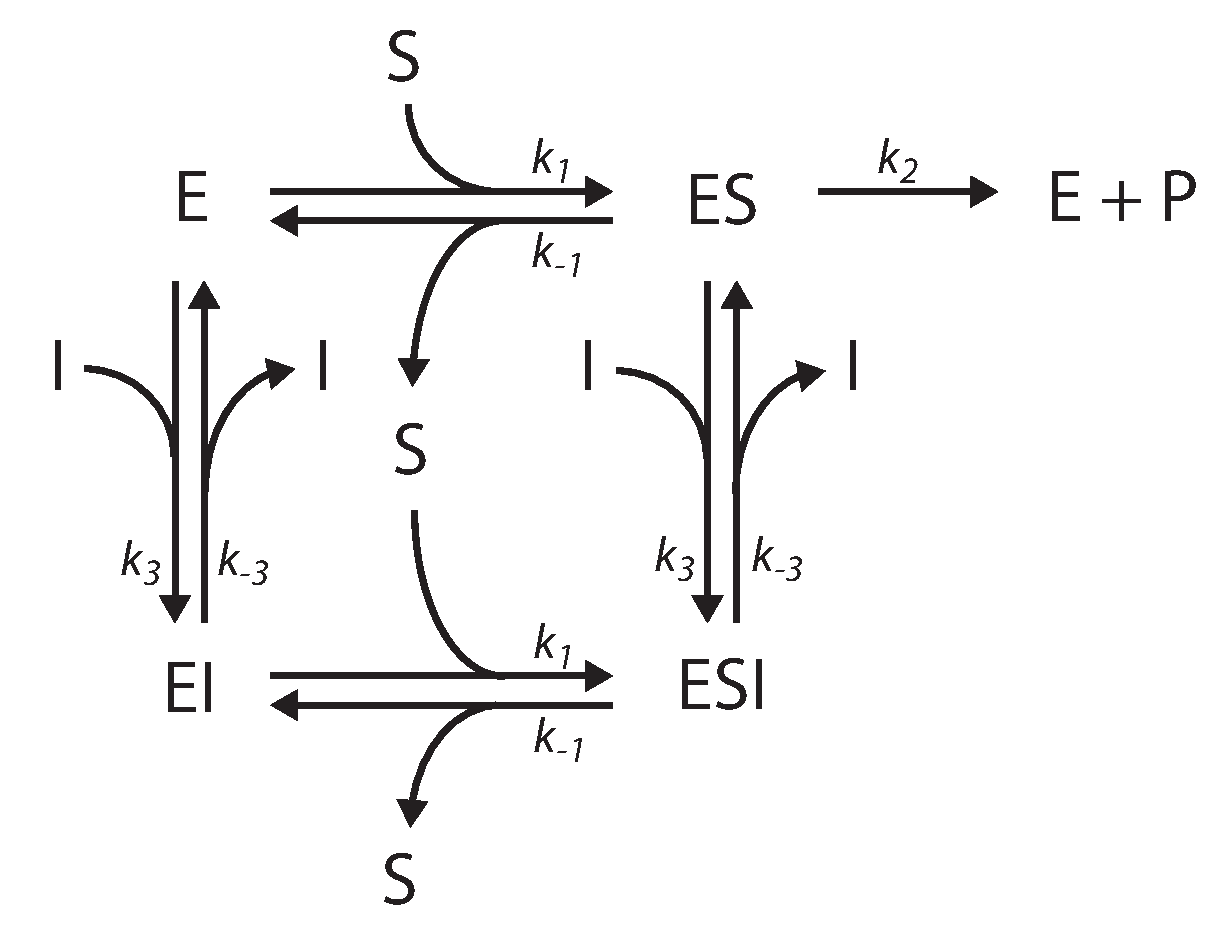
\includegraphics[width=0.4\textwidth]{non-competitive.pdf}}
\caption{Binding scheme for non-competitive inhibition.} \label{fig:noncompete}
\end{figure}  

By applying quasi-steady-state approximations to all three complexes and accounting for conservation of the enzyme moiety, show that:
\[\frac{d\left[ P \right]}{dt} = V = \left( \frac{V_{\textrm{max}}}{1 + \frac{\left[ I \right]}{K_I}} \right) \frac{\left[ S \right]}{\left[ S \right] + K_M } \]

\section*{Problem 3: Lineweaver-Burk Plots (30 points)}

$K_M$ and $V_{\textrm{max}}$ can be determined from measurements of the rate of product formation vs. initial substrate concentration. It is possible to estimate these values from a plot of production formation rate $V$ vs. substrate concentration $[S]$, but only if the substrate concentrations tested were chosen appropriatley.

\begin{enumerate}[a)]
\setlength{\itemsep}{0pt}
\item Describe how you would roughly estimate $K_M$ and $V_{\textrm{max}}$ for the data given in figure \ref{fig:mm}.
\end{enumerate}

\begin{figure}[htp] \centering{
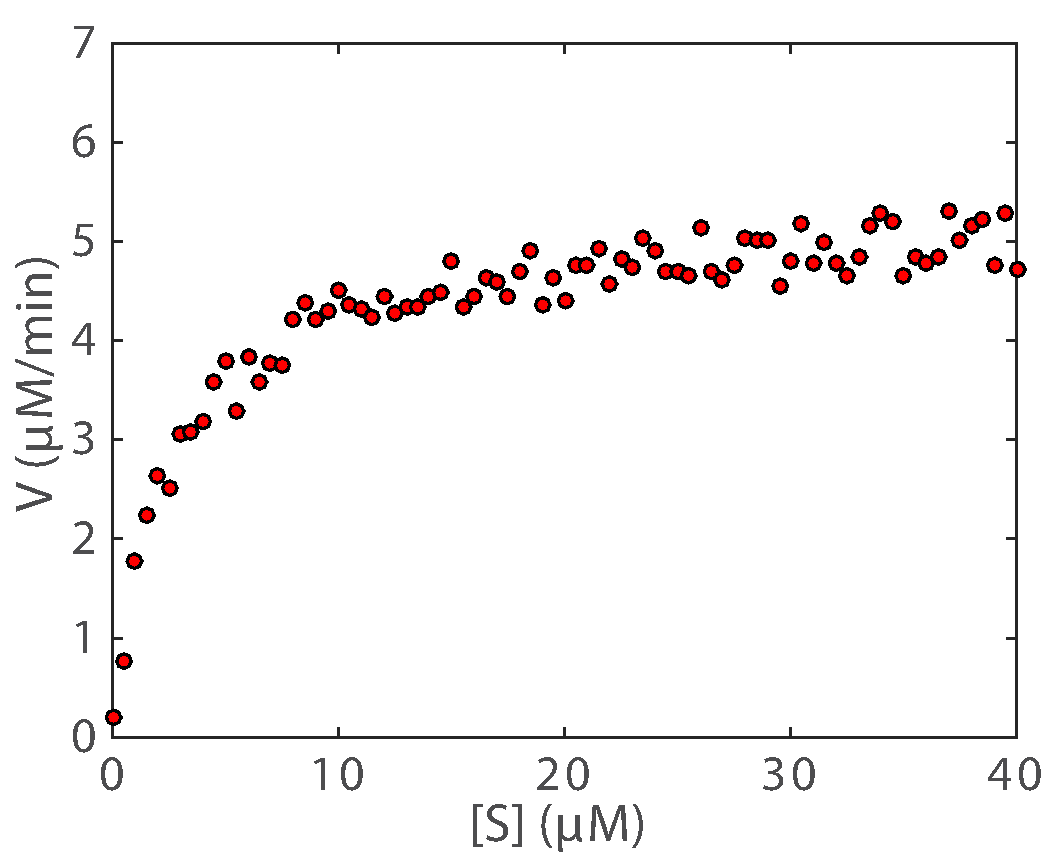
\includegraphics[width=0.4\textwidth]{mm_plot.pdf}}
\caption{An example plot of reaction rate vs. substrate concentration.} \label{fig:mm}
\end{figure}  

When this approach is not possible due to an inappropriate choice of data points or noise, $K_M$ and $V_{\textrm{max}}$ can still be estimated using a Lineweaver-Burk (aka double reciprocal) plot of $1/V$ vs. $1/[S]$.

\begin{enumerate}[a)]
\setlength{\itemsep}{0pt}
\setcounter{enumi}{1}
\item Rearrange the Michaelis-Menten expression,
\[ \frac{dP}{dt} = V = \frac{V_{\textrm{max}} \left[ S \right]}{K_M + \left[ S \right]}, \]
to find a linear expression for $1/V$ in terms of $1/[S]$. Describe how you can determine $K_M$ and $V_{\textrm{max}}$ from the slope and intercept of the line.
\item Lineweaver-Burk plots can also be used to determine the general mechanism of enzymatic inhibitors. Describe how you would expect the plot to differ in the presence vs. absence of:
\begin{enumerate}
\item A competitive inhibitor
\item A non-competitive inhibitor
\end{enumerate}
You may find it helpful to refer to the rate laws derived in problems 1 and 2.
\item Apply your approach to the data provided on the course website in the file \texttt{rate\_data.tsv}. Estimate $K_M$ and $V_{\textrm{max}}$ in the presence and absence of inhibitor. What type of inhibitor is this?
\end{enumerate}



\section*{Problem 4: Concerted Model of Cooperativity (Ingalls 3.7.11, 30 points)}

In 1965, Jacques Monod, Jeffries Wyman, and Jean-Pierre Changeux proposed a mechanistic model of cooperativity (Monod et al., 1965). Their model addresses a multimeric protein composed of identical subunits, each with one ligand binding site. They supposed that each subunit could transition between two conformations: a tensed state $T$ and a relaxed state $R$. For each protein molecule, all of the subunits are presumed to have the same conformation at any given time: transitions between the relaxed and tense states are \textit{concerted}.\\

In the absence of ligand, the tensed state is more stable than the relaxed state. The relaxed state, however, has a higher affinity for ligand. Thus, at a sufficiently high ligand concentration, ligand binding causes the protein to adopt the relaxed state. This increases the protein's affinity for ligand, triggering a positive feedback, and resulting in a sigmoidal binding curve.

\begin{figure}[htp] \centering{
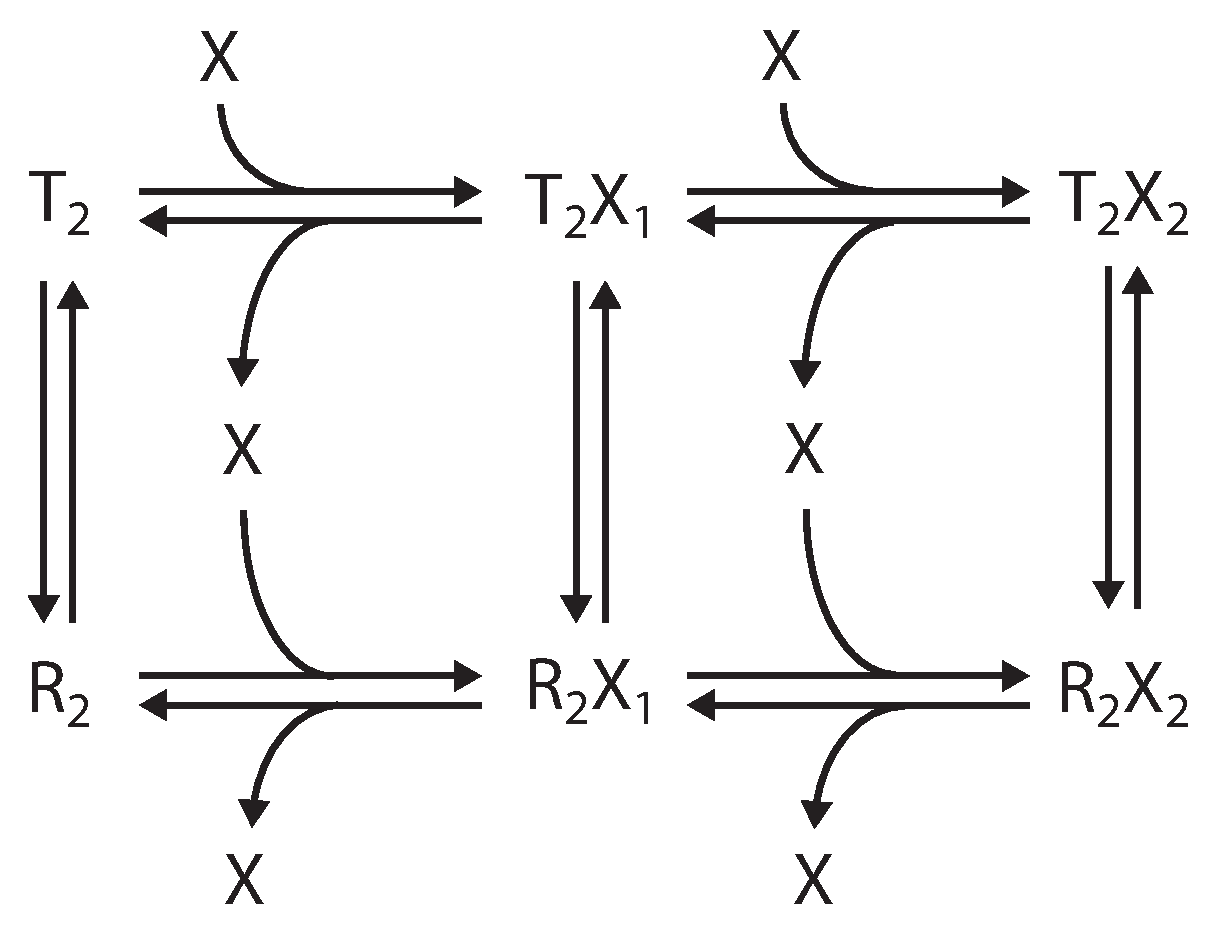
\includegraphics[width=0.4\textwidth]{ingallsmwc.pdf}}
\caption{Binding scheme for concerted model of cooperativity (Ingalls problem 3.7.11).} \label{fig:ingallsmwc}
\end{figure}  

This mechanism is called the \textit{MWC model}, or the \textit{concerted model}. The ligand binding scheme for a dimer is shown in figure \ref{fig:ingallsmwc}, where $R_2$ is the dimer of two relaxed monomers, and $T_2$ is the dimer of two tensed monomers.

\begin{enumerate}[a)]
\setlength{\itemsep}{0pt}
\item Let $K$ be the equilibrium constant for the $R_2 \leftrightarrow T_2$ conversion, i.e.:
\[  K = \frac{[T_2]}{[R_2]} \textrm{ at steady state} \]
Suppose that the dissociation constant for ligand binding to $R_2$ is $K_R$, and that the dissociation constant for ligand binding to $T_2$ is $K_T$. (The dissociation constants for the first and second binding event are the same, but the association/dissociation rates will depend on stoichiometry factors that reflect the number of sites.)\\

Confirm that in steady state, the concentrations satisfy
\begin{eqnarray*}
\left[ R_2 \right] = \frac{\left[ T_2 \right] }{K}  \hspace{ 2 cm} \left[ R_2X_1 \right] = \frac{2 \left[ X \right]  \left[ R_2 \right] }{K_R} \hspace{2 cm} \left[ R_2X_2 \right] = \frac{\left[ X \right]  \left[ R_2X_1 \right] }{2 K_R} \\
\left[ T_2X_1 \right] = \frac{2 \left[ X \right]  \left[ T_2 \right] }{K_T} \hspace{2 cm} \left[ T_2X_2 \right] = \frac{\left[ X \right]  \left[ T_2X_1 \right] }{2 K_T} \hspace{ 2 cm}
\end{eqnarray*}

(The stoichiometric prefactors reflect the availability of binding sites.) Use these equilibrium conditions to verify that in steady state, the fractional saturation is given by
\begin{eqnarray}
Y = \frac{K \frac{\left[ X \right]}{K_T} \left( 1 + \frac{\left[ X \right]}{K_T} \right) + \frac{\left[ X \right]}{K_R}  \left( 1 + \frac{\left[ X \right]}{K_R} \right) }{K \left( 1 + \frac{\left[ X \right]}{K_T}  \right)^2 + \left( 1 + \frac{\left[ X \right]}{K_R}  \right)^2} \label{eqn:fracsatmwc}
\end{eqnarray}

Plot the corresponding binding curves for $K_T = 1000$, $K_R = 1$, and $K = 500$, $1000$, and $2000$. Verify that although this is not a Hill function, the curves are nevertheless sigmoidal.
\item Consider the special case of the concerted mechanism in which $K=0$. Interpret the resulting binding mechanism and use formula \ref{eqn:fracsatmwc} to verify that the resulting binding curve is hyperbolic. Repeat for the case when $K_R = K_T$.
\item Verify that when the concerted model is applied to a tetramer (such as hemoglobin), the resulting fractional saturation is

\begin{eqnarray*}
Y = \frac{K \frac{\left[ X \right]}{K_T} \left( 1 + \frac{\left[ X \right]}{K_T} \right)^3 + \frac{\left[ X \right]}{K_R}  \left( 1 + \frac{\left[ X \right]}{K_R} \right)^3 }{K \left( 1 + \frac{\left[ X \right]}{K_T}  \right)^4 + \left( 1 + \frac{\left[ X \right]}{K_R}  \right)^4}
\end{eqnarray*}

\end{enumerate}

\end{document}